\chapter{System Build and Estimation}
\label{ch:estimate}

The two technologies are specified as equations and as constraints. This chapter turns the specification into a build that could host them, and then evaluates the equations on the field fixed in the problem set. Section~\ref{sec:build} is the system build: mechanical arrangement, sensors, computers, clocks and the software tasks that correspond to the blocks of Chapter~\ref{ch:design}. Section~\ref{sec:est} is the estimation: the protocol, the baselines, the numbers produced by the models, and the limits of what those numbers mean. The estimation does not contain a measurement that was not already implied by Table~\ref{tab:spec} and by Equations~\eqref{eq:openmiss}--\eqref{eq:work}. Where a sentence would be easier to read if it said ``the machine achieved'', the sentence says ``the model assigns''.

\section{System build}
\label{sec:build}

\subsection{Mechanical arrangement}

The chassis is a ladder of laminated softwood, two longitudinal members and three cross members, sized so that a four-row toolbar can be bolted on without a welded steel subframe as the primary structure. The Wood Handbook values for structural softwood are the design data for the members: modulus parallel to grain in the range used to justify a timber machine, and a check that moisture content is controlled before lamination so that the modulus assumed in \(k\) is the modulus the arm still has after a season \cite{woodhandbook}. Each row unit is a parallelogram. The two long links are timber. The pivots are steel pins in replaceable bushings, because a timber-on-timber pivot would frett and would change \(z_{\mathrm{bias}}\) faster than the filter's bias state is meant to follow. The boot is a short steel or cast opener on the timber link. Putting the wear surface in steel does not make the machine a steel planter. The compliance that moves the seed gate is still the timber link, and \(k=\SI{8200}{N/m}\) is the specification of that link, not of the boot.

The hopper on each row holds a single woody species, consistent with Assumption~\ref{as:seed}. It is a timber box with a polymer liner. The liner, not the wood, is the surface the seed slides on, so that pitch and dust do not change the friction the plate was tuned against. The plate has \(N=24\) cells, cut for the design seed, and is driven by a stepper through a reduction that can advance one cell pitch in the \(\tau_a=\SI{35}{ms}\) already charged to the repair law. If a vacuum plate is used instead of a mechanical cell, the same stepper drives the plate and a small blower holds the nominal \(\Delta p\) of Equation~\eqref{eq:vacuum}, including the vibration margin at the highest magnification allowed in \(\mathcal{V}_{\mathrm{meter}}\). The seed tube below the gate is wood-lined, of vertical drop \(H=\SI{0.42}{m}\), with a window for the lower camera view. A wooden tube is part of the object the detector must tolerate: the background is brown, and the augmentation practice of Blaser et al., who trained across light and viewpoint, is a requirement of the training set rather than an option \cite{blaser2024}.

The depth actuator is a linear screw on each row, rated for the \SI{120}{N} saturation used in the Lyapunov argument, with the \SI{80}{ms} lag of the model. It acts on the parallelogram and does not try to bend the timber link faster than the \SI{3}{Hz} bandwidth. Travel is set so that the \SI{18}{mm} target sits in the middle of the stroke, with enough extra stroke to remove the \SI{9.8}{mm} static deflection and to lift the boot clear of the soil in transport. Lift is a separate command. When the boot is up, the integral in Equation~\eqref{eq:depth} is frozen, as specified.

Row spacing is \SI{0.60}{m}, so four rows occupy the \SI{2.4}{m} swath used in the coverage arithmetic. The machine is drawn or self-propelled. The estimation uses a mass of \SI{460}{kg} and a wheelbase \(\ell\) inside the bicycle model, and it does not depend on which of those two traction arrangements supplies the force, because \(W_{\mathrm{mech}}\) is computed from resistance and slip rather than from an engine map. A self-propelled arrangement makes the speed command of the inner tracker a motor torque. A drawn arrangement makes it a request to the tractor. ISO~11783 is the request path in the drawn case \cite{iso11783}. In both cases the realised ground speed, not the request, is what Equation~\eqref{eq:plate} uses.

\begin{figure}[ht]
\centering
\begin{tikzpicture}[font=\small, >=Stealth, node distance=0.35cm]
  \node[draw, minimum width=10.2cm, minimum height=1.05cm, fill=brown!20] (frame) {laminated chassis, \SI{2.4}{m} toolbar};
  \node[draw, fill=brown!10, below left=0.6cm and -0.2cm of frame, minimum width=2.2cm, minimum height=0.9cm] (r1) {row 1};
  \node[draw, fill=brown!10, right=0.25cm of r1, minimum width=2.2cm, minimum height=0.9cm] (r2) {row 2};
  \node[draw, fill=brown!10, right=0.25cm of r2, minimum width=2.2cm, minimum height=0.9cm] (r3) {row 3};
  \node[draw, fill=brown!10, right=0.25cm of r3, minimum width=2.2cm, minimum height=0.9cm] (r4) {row 4};
  \node[draw, fill=blue!8, below=0.55cm of r2, minimum width=4.6cm, minimum height=0.85cm] (edge) {embedded computer, one detector thread per row};
  \node[draw, fill=orange!12, below=0.55cm of r3, minimum width=4.6cm, minimum height=0.85cm] (trk) {tracker computer, SCT-MPC at \SI{10}{Hz}};
  \draw[->] (r1.south) -- ++(0,-0.25) -| (edge.north);
  \draw[->] (r2.south) -- (edge.north);
  \draw[->] (r3.south) -- (trk.north);
  \draw[->] (r4.south) -- ++(0,-0.25) -| (trk.north);
  \draw[->] (edge) -- node[below, font=\scriptsize] {feasible \(v\)} (trk);
\end{tikzpicture}
\caption{Four-row build. Metering tasks stay on the row computers' detector threads. The tracker sees a feasible speed set and a realised speed, not a private copy of the plate state.}
\label{fig:build}
\end{figure}

\subsection{Sensors and the time base}

Each row carries one camera, one boot load cell, one ultrasonic range sensor and one inertial sensor. The camera frame is the observation the detector consumes. The load cell measures \(F_b\). The ultrasonic sensor measures \(r_u\). The inertial sensor measures the acceleration and the pitch rate that observe \(\ddot{\delta}\) and, by a known lever, \(\dot{\delta}\). A vehicle-level satellite and inertial navigation unit supplies \(x\), \(y\), \(\theta\) and \(v\) to the tracker. Centimetre-level satellite positioning is the class of fix Ehsani, Upadhyaya and Mattson used to map seed locations, and it is sufficient for a swath tracker at this speed \cite{ehsani2004}. It is not sufficient, by itself, to decide whether a cell was empty. That decision stays on the row camera.

All of these samples are useless to the filter if they do not share a clock. The build uses one clock domain. The tracker computer is the time master. Each row board disciplines its sampling to that clock over the same network that carries the feasible-speed message. A camera frame is stamped at exposure start, not at arrival of the image at the detector, because \(\tau_v\) is defined to include exposure. A plate command is stamped at the moment it is issued to the stepper. The difference between the exposure stamp of the frame that saw an empty cell and the issue stamp of the repair is the realised \(\tau_v+\tau_a\), and it is logged. If the realised delay exceeds the value assumed in Equation~\eqref{eq:vset} for more than a short burst, the row withdraws repair authority by lowering \(c\), which tightens \(\mathcal{V}_{\mathrm{meter}}\) from the machine rather than from the specification. This is the on-line honesty the Borja reversal requires: the inequality is checked with the delay the hardware is actually producing \cite{borja2018,borja2021}.

Table~\ref{tab:budget} is the timing budget the computers are required to meet. The numbers are allocations, and they sum to the latencies the control laws already use. A build that cannot meet an allocation has to change \(\mathcal{V}_{\mathrm{meter}}\) before it changes the law.

\begin{table}[ht]
\centering
\caption{Timing budget allocated to one row and to the vehicle tracker.}
\label{tab:budget}
\begin{tabular}{@{}lrr@{}}
\toprule
Task & Period & Budget \\
\midrule
Exposure and readout & \SI{33}{ms} frame & \SI{8}{ms} of \(\tau_v\) \\
Detector inference & per frame & \SI{14}{ms} of \(\tau_v\) \\
Filter update and plate law & \SI{10}{ms} & inside the remaining latency \\
Stepper execution of one pitch & on repair & \(\tau_a=\SI{35}{ms}\) \\
Depth servo & \SI{20}{ms} & bandwidth \SI{3}{Hz} \\
Feasible-set publish & \SI{100}{ms} & to the tracker \\
Tracker quadratic program & \SI{100}{ms} & finish inside \SI{40}{ms} \\
Heading replan & on request & seconds, off the hole period \\
\bottomrule
\end{tabular}
\end{table}

The detector budget of \SI{14}{ms} is plausible for a small model of the YOLOv10 class on an embedded graphics device, and it is not plausible for the class of microcontroller Borja used \cite{wang2024yolov10,borja2021}. The build therefore specifies an embedded graphics module per two rows, or one module with four threads and a hard preemption so that a slow frame on row~2 cannot borrow the \SI{14}{ms} of row~3. A frame that is still running at the deadline is cancelled. Cancellation is the dropped-frame rule of Section~\ref{sec:tech1}.

\subsection{Software tasks}

The software is a set of tasks with the periods in Table~\ref{tab:budget}, not a single loop. Bechar and Vigneault's subsystem split---sensing, decision, action, navigation---maps onto these tasks directly \cite{bechar2016}. Sensing is the camera and the analog acquisition. Decision on the row is Algorithm~\ref{alg:plate} and Equation~\eqref{eq:depth}. Action on the row is the stepper and the depth screw. Navigation is Algorithm~\ref{alg:outer} together with the quadratic program of Equation~\eqref{eq:stage}. The farm-scale record is a seed map: for each release, the filter's \(\hat{t}_{\mathrm{rel}}\), the vehicle pose at that time, and the estimated landing from Equation~\eqref{eq:carry}. Griepentrog and colleagues argued for exactly this record as the input to later weeding \cite{griepentrog2005}. A restoration planting uses it as the input to a later survival count, which is also the measurement that would one day replace the estimation function \(S(\sigma_z)\).

Task priorities follow the hole period. On each row the plate command outranks the depth servo, and the depth servo outranks logging. On the vehicle the quadratic program outranks a replan of heading. A replan that is still running when the machine is moving is discarded rather than applied half-computed, because a half-applied heading is not a heading the outer program evaluated. The tracker continues on the last feasible reference. This priority is the software form of Proposition~\ref{prop:feas}: feasibility of the current horizon is more important than optimality of the next heading.

The quadratic program is warm-started from the shifted previous solution, as the feasibility argument requires. qpOASES is the solver because it is an active-set method with a bounded, predictable cost on a problem of this size: fifteen steps, four states, two inputs, and linear inequalities \cite{ferreau2014}. A general nonlinear solver would also solve the problem and would not meet Requirement~R7 with the same predictability. CasADi is used off the machine to generate the Jacobian of the bicycle and the constraint matrices, and the generated evaluation is what runs at \SI{10}{Hz} \cite{andersson2019}. The estimation in the next section uses the same matrices in a direct evaluation of the outer cost. It does not need to simulate every quadratic-program step in order to rank headings, because Proposition~\ref{prop:feas} says that a reference inside the speed set is tracked without leaving the set. The estimation therefore ranks references by Equations~\eqref{eq:work}--\eqref{eq:mix}, and it treats tracking error as a separate, smaller contribution that does not reorder the headings.

\begin{figure}[ht]
\centering
\begin{tikzpicture}[x=0.78cm, font=\scriptsize, >=Stealth]
  \draw[->] (0,0) -- (14.2,0) node[below] {time};
  \foreach \x in {0,2,4,6,8,10,12} \draw (\x,0.05) -- (\x,-0.05) node[below] {\x0 ms};
  \draw[blue!70!black, line width=3pt] (0,1.0) -- (1.4,1.0) node[midway, above=2pt] {infer};
  \draw[blue!70!black, line width=3pt] (3.3,1.0) -- (4.7,1.0);
  \draw[blue!70!black, line width=3pt] (6.6,1.0) -- (8.0,1.0);
  \draw[orange!80!black, line width=3pt] (0.2,0.45) -- (1.0,0.45) node[midway, above=1pt] {QP};
  \draw[orange!80!black, line width=3pt] (10.2,0.45) -- (11.0,0.45);
  \node[anchor=west] at (0,1.55) {row detector, \SI{30}{Hz}};
  \node[anchor=west] at (0,-0.15) {};
  \node[anchor=east] at (0,0.45) {tracker};
\end{tikzpicture}
\caption{Two clocks. The row detector is fast enough to see every cell several times at the design speed. The tracker is an order of magnitude slower, which is the separation the joint problem was split along.}
\label{fig:clocks}
\end{figure}

\subsection{Safety interlocks}

A planter has a small number of states in which the correct command is to stop metering, and the build treats them as interlocks rather than as expensive regions of the cost. The plate is inhibited when the boot is lifted, when realised \(\tau_v+\tau_a\) exceeds the budget for longer than three hole periods, when the hopper-level sensor declares a row empty, and when the tracker reports that no speed inside \(\mathcal{V}_{\mathrm{meter}}\) is feasible on the current slope patch. The last of these is the situation Proposition~\ref{prop:feas} excludes on the design grade and includes on a grade or a roughness the specification did not see. Inhibiting the plate loses the rest of the swath and saves a resonant or a late-repair passage, which on the model of Figure~\ref{fig:qfi} is the right side of the cliff to stand on.

The depth screw is inhibited when the ultrasonic return is invalid for more than \SI{200}{ms}, and the last safe force is held. A held force is not a depth guarantee. It is a refusal to integrate noise. The vehicle is inhibited from entering the resonant speed interval even if a human operator overrides the working-speed set-point, unless a maintenance mode is selected with the plates disengaged. Override of a singulation constraint by a foot throttle is how a correct planner is turned back into the open-loop baseline. The interlock is unpopular and it is part of the technology.

\subsection{Interfaces between the two technologies}

Table~\ref{tab:iface} lists every quantity that crosses from one technology to the other. The list is short on purpose. A shared memory of filter covariances would couple the software releases of the row code and the tracker code, and it is not required by either algorithm.

\begin{table}[ht]
\centering
\caption{Quantities that cross the interface between the two technologies.}
\label{tab:iface}
\begin{tabularx}{\textwidth}{@{}l l X@{}}
\toprule
Quantity & Direction & Use \\
\midrule
\(\mathcal{V}_{\mathrm{meter}}\) & row to tracker & Hard constraint on \(v\) \\
Realised \(v\), \(a\) & tracker to row & Feedforward \(\omega^{\star}\) and the repair test \\
\(x_{\mathrm{ref}}(s)\) & prescription to both & Hole period and local feasible set \\
Release log & row to seed map & Later survival counts, not the live constraint \\
Realised delay & row to itself & Tightens \(c\) if the budget is missed \\
\bottomrule
\end{tabularx}
\end{table}

Nothing in the table is a learned weight. Replacing the detector with a later model changes \(\tau_v\) and the confidence calibration, and it does not change the tracker's quadratic program. Replacing the elevation model changes the outer search, and it does not change Equation~\eqref{eq:plate}. That replaceability is the practical form of the claim that the two technologies meet only at speed.

\subsection{Build sequence}

The build is staged so that a failure is attributable to one technology. The first stage is the timber row unit on a soil bin or a greased belt, with the vehicle speed simulated by the belt, as in the classical meter tests \cite{iso7256,panning2000}. At this stage \(\mathcal{V}_{\mathrm{meter}}\) is checked directly: repair success against hole period, and boot motion against a shaker set to \(\lambda\) and to speeds around \SI{2.4}{m/s}. The second stage connects two rows and looks for the common mode Assumption~\ref{as:flex} neglected. The third stage is the vehicle on a flat field, tracker only, plates disengaged, confirming that the quadratic program meets Table~\ref{tab:budget} and that the resonant interval is refused. The fourth stage is the joint system on the sloped field of the estimation, or on the nearest available slope, with the indices of Equation~\eqref{eq:qfi} measured by the same camera that the controller uses and by a second, recording camera that the controller does not see. The second camera is the check Zhao and colleagues used when they compared a detector with a high-speed recording \cite{zhao2025yolo}. The estimation in the next section is the prediction the fourth stage would be asked to confirm or to reject. It is not a substitute for that stage.

\section{Estimation}
\label{sec:est}

\subsection{Protocol}

The estimation evaluates the closed-form models on the field of Table~\ref{tab:spec}: \SI{80}{m} across the slope, \SI{180}{m} along the slope, grade \num{8}\%, area \num{1.44}~hectares. Swath width is \SI{2.4}{m}. Target spacing is \SI{0.20}{m}. The open-loop branch uses Equations~\eqref{eq:openmiss} and the open-loop half of Equation~\eqref{eq:deptherr}. The proposed branch uses Equations~\eqref{eq:cfrac}, \eqref{eq:closedmiss} and the closed-loop half of Equation~\eqref{eq:deptherr}, and it selects heading and speed by Algorithm~\ref{alg:outer}. Failure probability uses Equation~\eqref{eq:fail} with \(\kappa=1/2\) and \(S=\exp(-\sigma_z^2/(2\cdot 6.5^2))\) for \(\sigma_z\) in millimetres. Work uses Equations~\eqref{eq:fpm} and \eqref{eq:work} with the coefficients listed in Section~\ref{sec:tech2}. No coefficient is adjusted after the tables are seen. The script that evaluates the expressions is a direct transcription of those equations, so a change in a specification value changes the table in a way a reader can repeat.

Three plans are reported in every comparison.

\begin{enumerate}[label=\textbf{B\arabic*.}]
\item Open-loop plate, no depth servo, heading straight up the slope, steady speed \SI{1.6}{m/s}. This is the plan a careful operator might choose: long rows, a moderate speed, no electronics.
\item Open-loop plate, no depth servo, the same uphill heading, steady speed \SI{2.4}{m/s}. This is the plan that sits on the timber resonance in order to finish sooner.
\item The proposed pair of technologies. Heading and speed are whatever Algorithm~\ref{alg:outer} returns under the stated weights and under the index constraints.
\end{enumerate}

B1 and B2 are baselines in the sense of Requirement~R8. They use the same work model, the same field and the same flexure as B3. They differ in the metering branch and in the freedom to choose heading and speed. A comparison against a different field, or against a steel arm with a different \(f_n\), would mix those effects with the effect of the technologies.

\subsection{Speed response of the metering model}

Table~\ref{tab:speed} evaluates the metering model at zero acceleration, before any field geometry is applied. It is the numerical form of Figure~\ref{fig:qfi} together with the depth columns.

\begin{table}[ht]
\centering
\caption{Metering model at zero acceleration. Displacements are amplitudes or root-mean-square errors in millimetres. \(c\) is the repair fraction.}
\label{tab:speed}
\small
\begin{tabular}{@{}rrrrrrrrr@{}}
\toprule
\(v\) & \(f\) & \(M(r)\) & \(d\) & \(c\) & \(\qfi_{\mathrm{ol}}\) & \(\qfi_{\mathrm{cl}}\) & \(\sigma_{z,\mathrm{ol}}\) & \(\sigma_{z,\mathrm{cl}}\) \\
\midrule
0.8 & 1.78 & 1.11 & 4.07 & 1.00 & 0.904 & 0.983 & 5.71 & 1.68 \\
1.0 & 2.22 & 1.19 & 4.35 & 1.00 & 0.881 & 0.981 & 5.91 & 1.79 \\
1.2 & 2.67 & 1.30 & 4.74 & 1.00 & 0.858 & 0.980 & 6.21 & 1.93 \\
1.4 & 3.11 & 1.45 & 5.31 & 1.00 & 0.834 & 0.978 & 6.65 & 2.14 \\
1.6 & 3.56 & 1.68 & 6.15 & 1.00 & 0.809 & 0.976 & 7.33 & 2.65 \\
1.8 & 4.00 & 2.04 & 7.47 & 1.00 & 0.781 & 0.974 & 8.47 & 3.52 \\
2.0 & 4.44 & 2.66 & 9.73 & 0.80 & 0.750 & 0.927 & 10.52 & 5.00 \\
2.2 & 4.89 & 3.85 & 14.10 & 0.55 & 0.709 & 0.848 & 14.65 & 7.90 \\
2.4 & 5.33 & 5.92 & 21.64 & 0.33 & 0.653 & 0.752 & 22.01 & 13.20 \\
2.6 & 5.78 & 5.23 & 19.12 & 0.15 & 0.643 & 0.686 & 19.54 & 12.67 \\
2.8 & 6.22 & 3.10 & 11.34 & 0.15 & 0.657 & 0.697 & 12.03 & 8.15 \\
\bottomrule
\end{tabular}
\end{table}

Several facts in Table~\ref{tab:speed} are worth separating, because they have different consequences. From \SI{0.8}{m/s} to \SI{1.8}{m/s} the repair fraction stays at one and the closed-loop quality-of-feed index stays between \num{0.983} and \num{0.974}. The open-loop index over the same interval falls from \num{0.904} to \num{0.781}. The technology's benefit on count accuracy is therefore not a thin peak at one speed. It is a plateau. Depth tells a different story. Closed-loop depth error grows from \SI{1.68}{mm} to \SI{3.52}{mm} as the roughness frequency approaches the \SI{3}{Hz} servo bandwidth, and it is still inside the \SI{4}{mm} requirement at \SI{1.8}{m/s}. At \SI{2.0}{m/s} the latency margin starts to erode, \(c\) falls to \num{0.80}, closed-loop quality of feed drops to \num{0.927}, and depth error reaches \SI{5.00}{mm}. Both index constraints of the outer program fail together near that speed. The resonant row at \SI{2.4}{m/s} is worse than a smooth extrapolation of the plateau: dynamic displacement \SI{21.6}{mm}, open-loop depth error \SI{22.0}{mm}, and a closed-loop depth error of \SI{13.2}{mm} that shows, numerically, the content of Proposition~\ref{prop:split}. The servo was not given the bandwidth to remove a \SI{5.3}{Hz} motion, and the model does not pretend that it has.

The acceleration check at fixed \(v=\SI{1.8}{m/s}\) is the headland effect in isolation. At \(a=0\), \(0.4\), \(0.8\) and \(\SI{1.2}{m/s^2}\) the repair fraction is \num{1.00}, \num{0.98}, \num{0.85} and \num{0.71}, and the closed-loop miss probability is \num{0.010}, \num{0.014}, \num{0.041} and \num{0.072}. The constraint \(c\ge 0.85\) therefore bites between \num{0.8} and \(\SI{1.2}{m/s^2}\). The turn acceleration used in the field estimate, \(\SI{0.7}{m/s^2}\), sits just on the safe side of that bite at \SI{1.8}{m/s} and more comfortably on the safe side at the lower working speeds the optimiser actually selects.

\begin{figure}[ht]
\centering
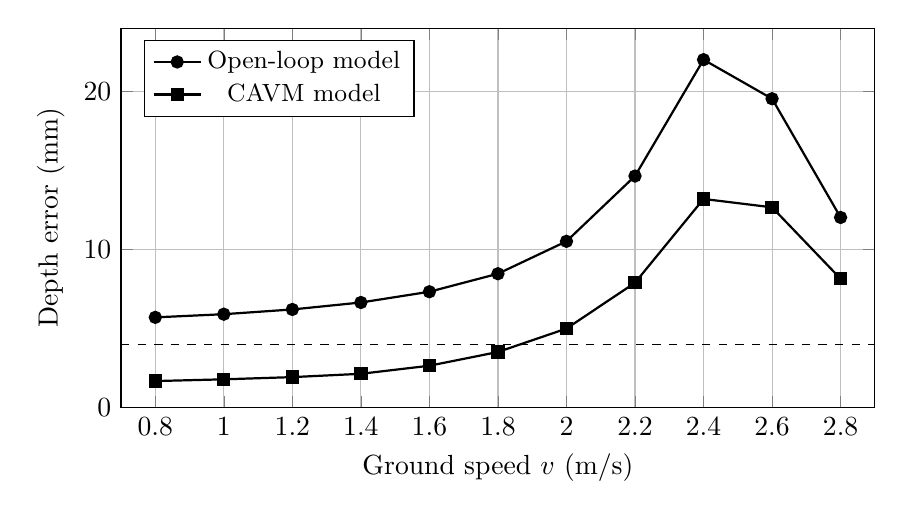
\begin{tikzpicture}
\begin{axis}[
  width=0.92\textwidth, height=6.4cm,
  xlabel={Ground speed \(v\) (m/s)},
  ylabel={Depth error (mm)},
  xmin=0.7, xmax=2.9, ymin=0, ymax=24,
  grid=both, legend pos=north west, legend style={font=\small}
]
\addplot[thick, mark=*] coordinates {
(0.8,5.71) (1.0,5.91) (1.2,6.21) (1.4,6.65) (1.6,7.33)
(1.8,8.47) (2.0,10.52) (2.2,14.65) (2.4,22.01) (2.6,19.54) (2.8,12.03)
};
\addplot[thick, mark=square*] coordinates {
(0.8,1.68) (1.0,1.79) (1.2,1.93) (1.4,2.14) (1.6,2.65)
(1.8,3.52) (2.0,5.00) (2.2,7.90) (2.4,13.20) (2.6,12.67) (2.8,8.15)
};
\draw[dashed] (axis cs:0.7,4) -- (axis cs:2.9,4);
\legend{Open-loop model, CAVM model, \SI{4}{mm} limit}
\end{axis}
\end{tikzpicture}
\caption{Modelled depth root-mean-square error. The dashed line is Requirement~R2. The peak is the timber resonance, which the speed set is required to avoid.}
\label{fig:depth}
\end{figure}

\subsection{Heading and speed on the estimation field}

Table~\ref{tab:field} applies the field geometry at four speeds that the metering plateau still regards as interesting. Energy changes little with speed, because aerodynamic drag is a small term beside rolling resistance at \SI{1}{m/s} to \SI{2}{m/s}. Energy changes more with heading. At \SI{1.5}{m/s} the uphill heading costs \SI{4.782}{MJ} and the best of the oblique headings shown, \ang{55} from uphill, costs \SI{4.416}{MJ}. The reduction is \((4.782-4.416)/4.782=\num{7.7}\%\). The pure contour costs \SI{4.451}{MJ}, slightly more than the \ang{55} heading, because the saving in grade loss is spent again on \num{75} turns against \num{48} turns. Time moves the other way: the contour takes \SI{1.455}{h} at this speed and the uphill heading takes \SI{1.289}{h}. Count accuracy at a given speed is almost indifferent to heading. The closed-loop quality-of-feed index at \SI{1.5}{m/s} is \num{0.977} on every heading in the table, and the accelerated fraction is only a few percent of the row. Heading is an energy and time decision inside the plateau. It becomes a singulation decision only when the accelerated fraction grows, which is the short-row, high-speed corner of the table.

\begin{table}[ht]
\centering
\caption{Field model with the closed-loop meter. Work is non-conservative mechanical work. The accelerated fraction \(\phi_{\mathrm{acc}}\) is the share of row length run at turn acceleration.}
\label{tab:field}
\small
\begin{tabular}{@{}llrrrrrr@{}}
\toprule
\(v\) & Heading & \(n\) & Work & Time & \(\phi_{\mathrm{acc}}\) & \(\qfi\) & \(\sigma_z\) \\
(m/s) & & & (MJ) & (h) & & & (mm) \\
\midrule
1.2 & uphill & 34 & 4.778 & 1.572 & 0.011 & 0.980 & 1.94 \\
1.2 & \ang{55} & 48 & 4.413 & 1.609 & 0.016 & 0.980 & 1.94 \\
1.2 & contour & 75 & 4.447 & 1.733 & 0.026 & 0.980 & 1.95 \\
1.5 & uphill & 34 & 4.782 & 1.289 & 0.018 & 0.977 & 2.36 \\
1.5 & \ang{55} & 48 & 4.416 & 1.331 & 0.026 & 0.977 & 2.36 \\
1.5 & contour & 75 & 4.451 & 1.455 & 0.040 & 0.977 & 2.37 \\
1.8 & uphill & 34 & 4.786 & 1.100 & 0.026 & 0.973 & 3.53 \\
1.8 & \ang{55} & 48 & 4.420 & 1.146 & 0.037 & 0.973 & 3.54 \\
1.8 & contour & 75 & 4.455 & 1.270 & 0.058 & 0.972 & 3.55 \\
2.0 & uphill & 34 & 4.789 & 1.006 & 0.032 & 0.924 & 5.02 \\
2.0 & \ang{55} & 48 & 4.423 & 1.053 & 0.046 & 0.923 & 5.03 \\
2.0 & contour & 75 & 4.458 & 1.177 & 0.071 & 0.921 & 5.05 \\
\bottomrule
\end{tabular}
\end{table}

Algorithm~\ref{alg:outer}, with the index filter \(\qfi\ge 0.955\) and \(\sigma_z\le\SI{4}{mm}\), and with the resonant interval removed, returns a heading of \ang{55} from uphill and a working speed of \SI{1.4}{m/s}. Neighbouring speeds inside the plateau are close in cost. The optimiser's preference for \SI{1.4}{m/s} rather than \SI{1.2}{m/s} is the time weight. Its refusal of \SI{1.8}{m/s} and above is the depth constraint, not the time weight: at \SI{1.8}{m/s} the depth error is still under \SI{4}{mm} in Table~\ref{tab:field}, and at the next step the filter fails. The preference for \ang{55} over the pure contour is the turn cost. The preference for \ang{55} over straight uphill is the grade term in Equation~\eqref{eq:fpm}. No single literature objective---minimum length, minimum energy, or minimum time---would have returned this pair by itself. Minimum time wants a higher speed and the uphill heading. Minimum energy on this rectangle wants a heading near \ang{55} to \ang{90} and is almost indifferent to speed. The singulation constraint is what keeps the speed on the plateau, and the turn term is what keeps the heading from sliding all the way to the contour.

\begin{table}[ht]
\centering
\caption{Plans compared on the estimation field. B3 is the proposed pair at the heading and speed Algorithm~\ref{alg:outer} returns.}
\label{tab:plans}
\begin{tabular}{@{}lrrrrr@{}}
\toprule
Plan & Work & Time & \(\qfi\) & \(\sigma_z\) & \(\rho_{\mathrm{fail}}\) \\
 & (MJ) & (h) & & (mm) & \\
\midrule
B1 open, uphill, \SI{1.6}{m/s} & 4.783 & 1.218 & 0.808 & 7.35 & 0.561 \\
B2 open, uphill, \SI{2.4}{m/s} & 4.797 & 0.864 & 0.652 & 22.04 & 0.998 \\
B3 proposed, \ang{55}, \SI{1.4}{m/s} & 4.415 & 1.410 & 0.978 & 2.15 & 0.068 \\
\bottomrule
\end{tabular}
\end{table}

Table~\ref{tab:plans} is the joint answer to Question~3. Against B1, the proposed plan reduces non-conservative work from \SI{4.783}{MJ} to \SI{4.415}{MJ}, which is \num{7.7}\%, and it reduces the modelled failure probability from \num{0.561} to \num{0.068}. The time cost of that reduction is real: \SI{1.410}{h} against \SI{1.218}{h}, about \num{16}\% longer than B1. Against B2, the proposed plan uses slightly less work, takes longer, and avoids a regime in which the model assigns a failure probability of \num{0.998}. The resonant plan is the fastest and, on this model, agronomically empty. The survival function is already below one half at a depth error of \SI{8}{mm} and is exhausted at \SI{22}{mm}. That conclusion is only as strong as \(S(\sigma_z)\). It is, however, the same functional form at every row of the table, so the ranking does not depend on a special choice made for B2 alone. B2 fails the depth requirement inside the open-loop model even before \(S\) is applied: \(\sigma_z=\SI{22}{mm}\) against a band of \(\pm\SI{8}{mm}\).

The work reduction of \num{7.7}\% sits a little below the \numrange{9.5}{15.6}\% direction savings Vahdanjoo, Gislum and S{\o}rensen reported, on different fields and with their own energy model \cite{vahdanjoo2023}. The present rectangle has a moderate grade and a slip coefficient that was chosen not to dominate rolling resistance. A steeper restoration slope would increase the gap between uphill and oblique headings and would make the energy term louder relative to the time term. It would not remove the resonant exclusion, which does not depend on grade. The \num{8.56}\% efficiency gain Xu, Lai, Guo and Lu found for a tracker allowed to pursue efficiency is a different quantity, measured against a pure tracking controller rather than against an uphill heading \cite{xu2022}. It is cited here as evidence that putting a non-tracking term inside a predictive tracker moves the result by an amount of this order, not as a number the present field is supposed to reproduce.

Seed count on B3 follows from the swath length. At \ang{55} the search uses a row length of \SI{125}{m} and \num{48} swaths, so the distance travelled while planting is \SI{6000}{m} per row and \SI{24000}{m} over four rows. At \SI{0.20}{m} spacing that is \(1.2\times 10^{5}\) seeds if every swath is full, which is the count \(N_{\mathrm{seed}}\) used to weight \(\rho_{\mathrm{fail}}\). A failure probability of \num{0.068} against \num{0.561} is a difference of about \(5.9\times 10^{4}\) seeds on that count. The figure is a model difference in failed placements, not a count of emerged seedlings. It is large because the open-loop depth error of \SI{7.35}{mm} already sits where \(S(\sigma_z)\) is falling steeply, and because the open-loop miss probability at \SI{1.6}{m/s} is \num{0.146}. Both contributions are visible in the formulae, and neither is a field emergence count.

\subsection{Where the gain comes from}

The gain splits into a part the first technology would produce on a fixed heading and a part that appears only when the heading is free. On the uphill heading at \SI{1.4}{m/s}, the closed-loop model already reaches \(\qfi=\num{0.978}\) and \(\sigma_z=\SI{2.15}{mm}\), with failure probability about \num{0.067}. That is almost the whole of the index gain of B3 over B1, and it is available without any coverage technology at all, at the price of the uphill work \SI{4.780}{MJ}. The coverage technology then moves the same metering performance onto a heading that costs \SI{4.415}{MJ}. Readers who want the singulation result without a new planner can stop at the first technology and a disciplined speed. Readers who want the work result need the second technology, and they only keep the singulation result if the planner is forbidden from spending the work saving on a higher speed. The joint design is the statement that the work saving will not be spent that way.

A further split, inside the first technology, separates the repair of empty cells from the depth servo. At \SI{1.4}{m/s} the open-loop miss probability from Equation~\eqref{eq:openmiss} is \num{0.125} and the closed-loop miss probability is \num{0.008}. That gap is the repair term, and it exists only while \(c=1\). The open-loop depth error is \SI{6.65}{mm} and the closed-loop depth error is \SI{2.14}{mm}. That gap is the servo, and Proposition~\ref{prop:split} says it will shrink if the machine is driven toward resonance. Table~\ref{tab:speed} at \SI{2.4}{m/s} is the shrinkage: the closed loop still improves depth relative to the open loop, from \SI{22.0}{mm} to \SI{13.2}{mm}, and \SI{13.2}{mm} is still a failed band. Vision metering without the speed constraint is not the technology that was specified. The tables that show a \num{0.978} index are tables in which the constraint is active as a restriction on the search, even though at the chosen point it is not active as a saturated inequality.

\subsection{Sensitivity the estimation can still speak about}

Three specification numbers have enough leverage that a reader will want to know the direction of a change, even though the estimation does not rerun a full identification.

If the equivalent stiffness is doubled, \(f_n\) rises by \(\sqrt{2}\) and the resonant speed for \(\lambda=\SI{0.45}{m}\) moves from about \SI{2.4}{m/s} to about \SI{3.4}{m/s}. The latency limit near \SI{1.9}{m/s} then binds before the resonance does. The forbidden interval moves out of the speeds a planter is likely to request, which is the steel-arm situation the introduction described. The depth servo still has to remove the static deflection, which would itself fall because \(k\) is larger. A stiffer arm makes the first technology easier and makes the resonance penalty in the tracker less often active. It does not retire the latency inequality. Borja's sign change did not require a wooden arm \cite{borja2021}.

If the detector slips from \SI{14}{ms} to \SI{40}{ms} of inference, \(\tau_v\) becomes \SI{48}{ms} and \(\tau\) becomes \SI{83}{ms}. The speed at which \(c\) remains \num{1} falls in proportion to the hole period. The plateau shrinks from the right. Algorithm~\ref{alg:outer} then returns a slower \(v_{\mathrm{work}}\), the time term grows, and the index constraints can still be met if any plateau remains. If the plateau disappears, the outer program returns no feasible candidate, which is a more honest outcome than a plan with a decorative camera. This is the microcontroller outcome, predicted by the same inequality that organised Section~\ref{sec:prev-meter}.

If the grade doubles and the slip coefficient stays put, \(\sin^2\alpha\) nearly quadruples because \(\alpha\) is small, and the work gap between uphill and oblique headings widens. The optimiser's preference for an oblique heading strengthens. The metering table does not move. A field trial on a steeper site would be expected to show a larger energy difference and the same speed ceiling, which is a falsifiable split between the two technologies.

If woody-seed detector recall is worse than the peanut and maize figures used in Equation~\eqref{eq:closedmiss}, every closed-loop miss probability rises. The estimation has no new image set with which to put a number on that rise. The direction is unambiguous, and it is the reason Assumption~\ref{as:est} forbids reading \num{0.978} as an expected field index for a named species. The build sequence in Section~\ref{sec:build} makes the belt test, not this table, the place where that index is first allowed to be empirical.

\subsection{Comparison with the nearest published systems}

A fair comparison states what was measured there and what is only modelled here. Borja's vision-assisted maize meter reduced missed hills at \SI{2}{km/h} and \SI{4}{km/h} and increased them at \SI{6}{km/h} \cite{borja2021}. The present model reproduces the shape of that reversal, through \(c(v,a)\), and moves the speed at which the reversal begins by assuming a \SI{22}{ms} vision budget instead of a microcontroller budget. It does not reproduce their hill counts. Mangus's electric-drive meter held a mean singulation of \num{98.45}\% over a wide speed range and lost accuracy when acceleration or seed rate rose \cite{mangus2017}. The present closed-loop plateau at \num{0.97} to \num{0.98} is a model expression of that kind of singulation, restricted to the speeds at which a repair can finish, and the acceleration term in Equation~\eqref{eq:openmiss} is a model expression of their acceleration finding. Blaser's and Zhao's detectors supply the error rates the repair formula is allowed to believe \cite{blaser2024,zhao2025yolo}. They do not supply a wooden tube in the training set.

On the planning side, Vahdanjoo, Gislum and S{\o}rensen showed that a three-dimensional energy criterion moves the preferred seeding direction by enough to matter \cite{vahdanjoo2023}. The oblique heading in Table~\ref{tab:plans} is the same kind of decision, on a simpler elevation model, with extra constraints. Zhang and colleagues' seeding-robot planner reports a missed-sowing rate of \num{1.8}\% together with a large energy reduction in their own trials \cite{zhang2025path}. The present model at B3 assigns a miss probability near \num{0.008} on the plateau, which is a lower miss rate than \num{1.8}\% and is not a competing experimental claim. It is a statement that, if the detector and the stepper perform as the repair formula assumes, empty-cell misses are almost removed and the remaining failure is depth and the occasional multiple. Their planner and this one can be combined: their search can carry Equation~\eqref{eq:fail} as an edge cost, and the inner tracker of this thesis can track the path they return, provided the path's speed profile is projected onto \(\mathcal{V}_{\mathrm{meter}}\) before tracking begins.

No published system reviewed in Chapter~\ref{ch:previous} closes the loop from a timber natural frequency to a coverage constraint. That closure, rather than a new record on maize singulation, is the comparison this estimation is built to illustrate.

\subsection{Limits}

The limits are the assumptions, restated against the tables so that the largest numbers in the chapter stay attached to them.

The failure probabilities inherit \(S(\sigma_z)\) and \(\kappa=1/2\). A species whose emergence is tolerant of a \SI{7}{mm} depth error would shrink the gap between B1 and B3. A species as intolerant as the spinifex in Masarei, Guzzomi, Merritt and Erickson's trial would enlarge it and would also force a smaller \(\sigma_{z,\max}\) than \SI{4}{mm} \cite{masarei2019}. The design case at \SI{18}{mm} with an \SI{8}{mm} band is neither of those species.

The open-loop intercepts in Equation~\eqref{eq:openmiss} were chosen to sit in a plausible band for irregular seed. A plate that has already been tuned for the woody species might start from a better open-loop index, and the vision benefit on misses would then be smaller. The resonant depth peak would remain, because it is produced by \(M(r)\) and by the \SI{4}{mm} unresolved bias, not by the miss intercept.

Chassis coupling, mixed species, wheel slip beyond the force model, and detector performance on a dusty wooden tube are outside the numerical evaluation. The build sequence is where they stop being outside the project. Until that sequence is run, Table~\ref{tab:plans} is a comparison of plans under a declared model. It is evidence that the constraints are coherent and that they bind in the right places: latency at one speed, resonance at another, grade and turns in the heading. It is not evidence that a particular laminated arm has \(k=\SI{8200}{N/m}\), and it is not evidence that a stand of woody seedlings will emerge in the ratio \(1-0.068\).

\subsection{Checking the selected plan against the requirements}

Requirement~R8 asked for the baselines to sit in the same table as the proposal, and Table~\ref{tab:plans} is that table. The other requirements can be checked on B3 without a further search. The closed-loop quality-of-feed index at the selected point is \num{0.978}, which clears R1's floor of \num{0.95}. The depth error is \SI{2.15}{mm}, which clears R2's ceiling of \SI{4}{mm}. The speed \SI{1.4}{m/s} lies inside the full-repair side of Equation~\eqref{eq:latency}, so R3 is met as a constraint that discarded faster candidates rather than as a penalty the weights happened to respect. The resonant interval is not the selected speed, and it is not inside \(\mathcal{V}_{\mathrm{meter}}\), so R4 holds for the plan even though a human override could still violate it if the interlock in Section~\ref{sec:build} were omitted. The cost that ranked \ang{55} above uphill and above the pure contour contains work, time and \(\rho_{\mathrm{fail}}\), and \(\rho_{\mathrm{fail}}\) uses the closed-loop miss model, so R5 holds. Four independent row tasks are in the build, so R6 holds as an architectural requirement the estimation's single-row formulas do not by themselves prove. The tracker period and the quadratic program are specified, so R7 holds as a budget, not as a measured solve time. The language of the tables is model language, so R9 holds if the surrounding prose is read with the tables. One speed set is published by the meter and consumed by the tracker, so R10 holds by the interface in Table~\ref{tab:iface} and by the prescription example in which a shorter spacing moves that same set.

The check is worth doing explicitly because a plan can win a table and still break a requirement that was never a column. B2, for example, wins the time column and fails R1, R2 and R4 at once. B1 meets none of the index requirements and was never required to: it is the baseline those requirements are measured against. B3 is the only one of the three that is feasible for the joint problem as Definition~\ref{def:p3} stated it. That is a stronger statement than ``B3 has the smallest failure probability'', and it is the statement the requirement list was written to support.

\subsection{A measurement sheet for the fourth build stage}

The fourth stage of the build is the first moment at which Table~\ref{tab:plans} could be wrong in the empirical sense. The sheet below is the comparison that stage should record, so that a disagreement has an address. Each row is one operating point already present in the model tables. The recording camera, not the control camera, supplies \(\qfi\), \(\mis\) and \(\mul\) by the classification of Equation~\eqref{eq:classes} on at least five hundred spacings, which is the order of count at which a miss rate of one percent is distinguishable from a miss rate of three percent. Depth is the mean and the root-mean-square of boot penetration against the \SI{18}{mm} target, measured by the ultrasonic sensor and, on a calibration strip, by a manual check of uncovered seed. Work is not measured as a germination count. It is measured as drawbar pull or as motor current integrated over a swath of known length, on the uphill heading and on the \ang{55} heading, at the same speed, so that the \num{7.7}\% gap has a chance to appear or to fail without being mixed with a speed change.

\begin{table}[ht]
\centering
\caption{Points the field stage should record beside the model. Model columns repeat Chapter~2 and this chapter. The empty columns are the measurement.}
\label{tab:sheet}
\small
\begin{tabular}{@{}llrrrr@{}}
\toprule
Point & Quantity & Model & Recorded & Unit & Pass if \\
\midrule
\(v=\SI{1.4}{m/s}\), straight & \(\qfi_{\mathrm{cl}}\) & 0.978 & & -- & \(\ge 0.95\) \\
\(v=\SI{1.4}{m/s}\), straight & \(\sigma_z\) & 2.15 & & mm & \(\le 4\) \\
\(v=\SI{1.4}{m/s}\), \(a=\SI{0.7}{m/s^2}\) & \(c\) stays high & yes & & -- & repairs still timely \\
\(v=\SI{2.4}{m/s}\), straight & \(\sigma_{z,\mathrm{ol}}\) & 22 & & mm & resonance visible \\
\(v=\SI{2.4}{m/s}\), commanded & speed refused & yes & & -- & interlock holds \\
uphill versus \ang{55} & work gap & 7.7 & & \% & same sign \\
realised delay & \(\tau_v+\tau_a\) & 57 & & ms & budget holds \\
\bottomrule
\end{tabular}
\end{table}

Two outcomes of that sheet would change the design rather than only the numbers. If the resonant peak is absent, \(k\) or \(\lambda\) differs from the specification and the forbidden interval should be recomputed from the measured frequency, not deleted from the tracker on the strength of one smooth run. A single run can miss a wavelength. If the resonant peak is present and the closed-loop depth error at \SI{1.4}{m/s} is nevertheless above \SI{4}{mm}, the servo bandwidth or the bias estimate is wrong and Proposition~\ref{prop:split} still stands: the remedy is not to drive faster. If realised delay is near \SI{100}{ms}, the plateau shrinks and Algorithm~\ref{alg:outer} must be rerun with the new \(\tau\) before any claim about \SI{1.4}{m/s} is repeated. If the work gap changes sign, the slip coefficient or the grade of the site is not the one in Equation~\eqref{eq:fpm}, and the heading search should be rerun with the measured resistance. In every one of those cases the structure of the two technologies stays. What moves is a specification value that the estimation, by construction, held fixed.

The sheet also records what a negative singulation result would mean. A quality-of-feed index of \num{0.90} at \SI{1.4}{m/s} with a healthy delay budget would say that Equation~\eqref{eq:closedmiss} was optimistic about detector recall on this seed, which Assumption~\ref{as:est} already flagged. The speed constraint would remain, because it did not depend on the recall figure. The depth loop would remain, because it does not use the detector. The coverage ranking of headings would remain, because inside the plateau the miss rate barely changes with heading. The number \num{0.978} would be retired. The architecture would not. That separation is the useful product of having written the model in pieces that can fail separately.

\subsection{A short spacing tape, scored by hand}

The indices are easier to trust after they have been scored once by hand, on a tape short enough to add up. Suppose twenty successive spacings, in millimetres, are recorded on the belt at the design target of \SI{200}{mm}:
\begin{equation*}
\begin{aligned}
&210,\; 190,\; 205,\; 90,\; 310,\; 200,\; 198,\; 202,\; 215,\; 185,\\
&400,\; 188,\; 207,\; 195,\; 220,\; 70,\; 130,\; 203,\; 197,\; 208.
\end{aligned}
\end{equation*}
The class boundaries are \SI{100}{mm} and \SI{300}{mm}. The value \SI{90}{mm} is a multiple. The value \SI{310}{mm} that follows it is what a double often leaves behind, and it is a miss. The value \SI{400}{mm} is a miss. The pair \SI{70}{mm} and \SI{130}{mm} contains one multiple; \SI{130}{mm} is a single because it clears half the target. Sixteen spacings are singles. Then \(N_{\mathrm{tot}}=20\), \(N_u=2\), \(N_m=2\), \(N_s=16\), and
\begin{equation}
\label{eq:hand}
\qfi = 0.80,\qquad \mul = 0.10,\qquad \mis = 0.10.
\end{equation}
The single-class mean and the coefficient of variation use only those sixteen singles, not the \SI{90}{mm} or the \SI{400}{mm}. Including those two would inflate the coefficient of variation and would hide, inside one number, the fact that most seeds were close to the target and two events were categorical failures. That is the distinction Kachman and Smith insisted on, and it is why the estimation reports \(\qfi\), \(\mis\), \(\mul\) and a depth error rather than one coefficient of variation for the whole tape \cite{kachman1995}. A field stage that published only a coefficient of variation would not be able to confirm or reject Table~\ref{tab:plans}.

Twenty spacings are an illustration, not a sample size. Five hundred spacings, as the measurement sheet asks, make a miss rate of \num{0.01} a handful of events and a miss rate of \num{0.15}, the open-loop model at \SI{1.6}{m/s}, a hundred and fifty events. Those two samples cannot be confused. The estimation's claim that B3 and B1 are different is a claim about that separation under the model. The tape shows the arithmetic the field stage must not replace with a smoother and less informative summary.

\subsection{Reading the energy prize at the scale of one hectare}

The \SI{0.37}{MJ} difference between B1 and B3 is \SI{0.10}{kWh}. On a \num{1.44}~hectare field that is a small energy quantity beside the fuel a truck spends to deliver the machine, and it is the right order of magnitude for a direction choice on a moderate grade. Reported direction savings of \numrange{9.5}{15.6}\% on other seeding fields are the same kind of quantity: a fraction of an already-modest in-field energy, not a new power source \cite{vahdanjoo2023}. The estimation would mislead a reader who remembered only the percentage and forgot the base. \num{7.7}\% of \SI{4.78}{MJ} is the prize. The singulation and depth columns are where the technologies change the operation by a factor rather than by a fraction. Failure probability falls from \num{0.561} to \num{0.068}, a factor of about eight, under a survival function that treats a \SI{7}{mm} depth error as already serious. Even if a later germination trial halves that factor, the index gap remains the reason to build the vision loop, and the energy gap remains a constraint on how the planner is allowed to spend the time the loop requires.

Per hectare, using \(1.44\)~ha as the divisor, B3 uses about \SI{3.07}{MJ/ha} and about \SI{0.98}{h/ha}, and it assigns a failed-placement fraction of \num{0.068}. B1 uses about \SI{3.32}{MJ/ha} and about \SI{0.85}{h/ha}, with a failed-placement fraction of \num{0.561}. A contractor who bills only time will prefer B1 and will plant a stand the model regards as mostly outside the depth band. A contractor who bills for established plants, which is the usual contract in restoration, will prefer B3 even before the energy line is read. Pedersen, Fountas, Have and Blackmore made the same structural point for agricultural robots in general: the robot pays when the operation it enables is one the cheaper machine misses, not when it is a few percent cheaper at the same operation \cite{pedersen2006}. The wooden planter with these two technologies is in that category if, and only if, the depth and singulation gaps survive the measurement sheet. The energy line is not the category.

\subsection{The same rectangle turned the other way}

The estimation field was chosen so that a contour heading has short rows. That choice is doing real work, and it should be shown by computing the opposite geometry with the same equations and the same coefficients. Turn the rectangle so that the long side, \SI{180}{m}, lies on the contour and the short side, \SI{80}{m}, runs up the \num{8}\% grade. At \SI{1.4}{m/s} the work model then assigns \SI{4.16}{MJ} and \SI{1.37}{h} to the contour heading, with \num{34} turns, and \SI{5.12}{MJ} and \SI{1.53}{h} to the uphill heading, with \num{75} turns. Contour travel is cheaper per metre because \(\Gamma(\ang{90})=1\), and it is also shorter in time because the long rows cut the number of turns. Both terms agree. Algorithm~\ref{alg:outer} and a planner that minimises only work return the same heading. The singulation constraint still chooses the speed, because nothing in the rotation moves \(f_n\) or \(\tau\), and the selected speed remains \SI{1.4}{m/s} on the plateau of Figure~\ref{fig:qfi}.

On the original field the agreement breaks. Uphill travel at \SI{1.4}{m/s} costs \SI{4.78}{MJ} and \SI{1.37}{h}. Contour travel costs \SI{4.45}{MJ} and \SI{1.53}{h}. The \ang{55} heading returned by the joint search costs \SI{4.41}{MJ} and \SI{1.41}{h}. Pure minimum work and the joint search are close, and they are not identical: the turn term and the time weight pull the optimum off the pure contour, by a few tenths of a megajoule, toward a longer row. A reader who only remembers that ``the planner chose an oblique heading'' has missed the smaller and more useful fact. The oblique heading is the compromise on a field that punishes the contour with turns. On a field that rewards the contour with both energy and time, the compromise disappears and the constraint that remains is the speed ceiling from the wooden arm and the vision budget. The two technologies are still both active. One of them has nothing left to trade.

This rotation is the last numerical check the estimation makes. It uses no new coefficient. It shows that the heading result in Table~\ref{tab:plans} is a property of the field orientation fixed in the problem set, not a universal preference for \ang{55}. The speed result is the one that travels. Wherever the long side points, steady running stays off the resonance and inside the repair inequality, or the outer program returns no plan.

Within those limits the estimation answers the three research questions in the only sense a design thesis can answer them before a prototype. The plate law and the flexure filter of Section~\ref{sec:tech1} repair empty cells only while the repair fraction is high, and they assign mean depth to a servo whose bandwidth sits below \(f_n\). The outer search and the inner quadratic program of Section~\ref{sec:tech2} select a heading and a speed inside that repair set, with grade work, turn time and failed placements in one cost. On the estimation field the selected plan is \ang{55} from uphill at \SI{1.4}{m/s}, with modelled quality of feed \num{0.978}, depth error \SI{2.15}{mm} and non-conservative work \num{7.7}\% below the uphill open-loop plan at \SI{1.6}{m/s}. The resonant open-loop plan is faster and, in the same model, does not establish the crop. The prototype specified in Section~\ref{sec:build} is the instrument that would turn these statements into measurements.
